
% simple.tex - A simple article to illustrate document structure.

% preamble

\documentclass{article}

%% \usepackage{times}
\usepackage{latexsym}
\usepackage{url}
\usepackage{hyperref}
\hypersetup{colorlinks=true}
\usepackage{graphicx}

\begin{document}

% top matter

\title{Algorithm Design Project: 
\newline
MineSweeper Game and Auto-solver}

\author{Efrem \c{S}tefan \and Hagiu Teodora}
\date {5th June 2018}
\maketitle
\item{Computer Science English Section First Year Group 1.1 A}

\begin{tabbing}
\indent{Course Professor: }{ Costin Badica} \\
\indent{Laboratory Professor: }{ Alex Becheru} \\

\end{tabbing}

\pagebreak


% sections
\section{Problem statement}
The MineSweeper Game: a program that allows you to play the game yourself on a board of 16x16 spaces with 40 mines and the auto-solver for the game given the first move. The game consists in a board that has mines placed randomly on it and the goal is to find all the places that don't contain a mine.

\linebreak


\section{Application Design}


\begin{itemize}
  \item The application uses one main function where we call the start game auxiliary function and 9 auxiliary functions called in the start game function and other functions in order to make the whole program more organized.
 
  \end{itemize}
  
  \item The main function is represented by :
  
  \begin{itemize}
  \item The use of auxiliary function start game.
  \end{itemize}
  
  \item The auxiliary functions for the game are:
  
  \begin{itemize}
   \item Build mines board function
        \begin{itemize}
            \item It creates a char matrix and puts the mines randomly in it
            \item After the mines have been placed, it puts numbers with how many mines are around a space in the matrix using the auxiliary function increment.
        \end{itemize}
   \item Print mines board function.
        \begin{itemize}
            \item This function prints the mines board matrix when you lose the game.
        \end{itemize}
   
   \item Increment function
        \begin{itemize}
            \item The function adds 1 at the space given.
        \end{itemize}
   
   \item Build player board function
        \begin{itemize}
            \item The function creates the player board matrix, the matrix that you see and use to see your moves.
        \end{itemize}
   
   \item Print player board function
   
    \begin{itemize}
        \item The function prints the player board matrix after every move you make, to see the changes done.
        \end{itemize}
   
   \item Reveal spaces function
        \begin{itemize}
            \item The function reveals the space you chose and if that space is a 0 on the mines board ( with no mine around it) it reaveals all blank the spaces around it until it gets to the ones with mines around.
        \end{itemize}
   
   \item Loss function
        \begin{itemize}
            \item In case you hit a mine, this function shows you a loss message and asks you if you want to play again and in the case you do want, it calls the function start game again.
        \end{itemize}
   
   \item Win function 
        \begin{itemize}
            \item In case you win the game this function shows a win message and asks you if you want to play again and in the case you do want, it calls the function start game again.
        \end{itemize}
   
   \item Check win function 
        \begin{itemize}
            \item At every step you make, this function checks if you won the game (no spaces without a mine on them left) and returns TRUE (1) in case the game is finished and FALSE(0) otherwise.
        \end{itemize}
   
   \item Start Game function
        \begin{itemize} 
            \item The build mines board and build player board are called.
            \item The player board matrix is printed with the function print player board
            \item A welcome message is printed along with the legend (the meaning of each character and number that appears).
            \item With the help of  variable decision (given by the player in the input) the function clears a space with the help of reveal spaces function or marks it with a M that stands for mine.
            \item The player board with the new changes is printed.
            \item With the use of check win function, at every step the win condition is checked, and if it is true the win function is called.
        \end{itemize}
     
   
       
        
 Besides the ones presented above, the auxiliary functions used in the auto-solver are:
    \item Build solver chance board function
        \begin{itemize}
        \item It creates an int matrix where it stores the chances for a space to be a mine.This function is used in the start game function next to build player board and build mines board.
        \end{itemize}
        
    \item Print solver chance board function
        \begin{itemize}
        \item This function prints the solver chance board. It was used just for tests or to see how the program works.
        \end{itemize}
        
    \item Look for mines function
        \begin{itemize}
        \item Given a space on the board this function searches around to see how many mines and hidden spaces are. If the number of mines is equal to the number of the current space, it reveals all the other hidden spaces around. If the number of hidden spaces is equal to the number of the current space minus the number of mines found, it marks all the hidden spaces with M for mines.
        \end{itemize}
        
    \item Automatic flagging function
        \begin{itemize}
        \item This function goes through all the revealed numbers on the board and calls the look for mines function to reveal spaces around or mark the mines.
        \end{itemize}
        
     \item Automatic chance placer function
        \begin{itemize}
        \item The function goes through all the hidden spaces and calls the function place chance to see the chances.
        \end{itemize}
        
     \item Place chance function
        \begin{itemize}
        \item The function stores the chances for a space to be a mine in the solver chance board and adds the numbers of the revealed spaces around.
        \end{itemize}
        
     \item Automatic decision taker function
        \begin{itemize}
        \item The function goes through the spaces and searches for the one with the minimum chance (minimum number) and reveals it.
        \end{itemize}
        
        
     \item Start Game function
        \begin{itemize} 
            \item The build mines board, build solver chance board and build player board functions are called.
            \item The player board matrix is printed with the function print player board
            \item A welcome message is printed along with the asking of the first move ( the row and the column of the space you want to start from) 
            \item With the help of  variable step (given by the player in the input) the program shows every step done to get to the final (the variable needs to be given after each step as a confirmation).
            \item The player board with the new changes is printed
            \item With the use of check win function, at every step the win condition is checked, and if it is true the win function is called.
        \end{itemize}
    


        
    
\subsection{Input Specification:}

The input is given by the player and it is needed at every step. It consists in the decision, the row and the column of the space.

\subsection{Output Specification.}

The output consists in multiple prints of the player board matrix at every step made and finally the win ore lose messages along with the mines board matrix (in the case of a loss).
    
    
\item The list of all files in the application and their description for the game:
 \begin{itemize}
 	\item minesweeper\_game.c: the main file in which we create the application.Here we declare the libraries and headers.
 	\item pre\_game\_boards.c: the file in which the functions used for building and printing the matrices and the increment function are stored..
 	\item pre\_game\_boards.h : the header file in which the functions used for building and printing the matrices and the increment functions are declared.
 	\item in\_game\_functions\_player.c : the file in which the functions reveal spaces, win, lose, check win and start game are stored.
 	\item in\_game\_functions\_player.h : the header file in which the functions reveal spaces, win, lose, check win and start game are declared.
 	
 \end{itemize}
 
 
 \item The list of all files in the application and their description for the auto-solver:
 \begin{itemize}
 	\item autosolvermsp.c: the main file in which we create the application.Here we declare the libraries and headers.
 	
 	\item pre\_game\_boards.c: the file in which the functions used for building and printing the matrices and the increment function are stored.
 	
 	\item pre\_game\_boards.h : the header file in which the functions used for building and printing the matrices and the increment function are declared.
 	
 	\item pre\_game\_autosolver\_boards.c : the file in which the functions used for building and printing the matrix that helps to keep the chances for a mine are stored.
 	
 	\item pre\_game\_autosolver\_boards.h : the file in which the functions used for building and printing the matrix that helps to keep the chances for a mine are declared.
 	
 	\item in\_game\_functions\_autosolver.c : the file in which the functions reveal spaces, win, lose, check win, look for mines, automatic flagging, automatic chance placer, place chance, automatic decision taker and start game are stored.
 	
 	\item in\_game\_functions\_autosolver.h : the header file in which the functions reveal spaces, win, lose, check win, look for mines, automatic flagging, automatic chance placer, place chance, automatic decision taker and start game are declared.
 	
 \end{itemize}
   
      \end{itemize}
  
 


\section{Conclusions}


\subsection{Achievements}

Firstly, we achieved learning more about the game we play when we are bored and have some minutes. Secondly, we consider that this project was one of the most interesting ones, and that's why we decided to stick to it. We also have learned more about using LaTeX as a documentation method, and we are looking forward in new projects, interactive like this one where we learned how to think the game better and keep it simple at the same time.
\linebreak

\subsection{Challenging parts}

One of the interesting parts in the development process of the project was building the skeleton of the application, which needed a lot of patience and finally no one was harmed, even if code didn't work sometimes.It's the first time when we create a legit project with more than one .c file, so it was really interesting and fun and we also learned a lot.
\newline

Another interesting part of the project was learning how to use LaTeX as a documentation method, how to use DoxyGen as a comment extractor and see how the game we play so much works in the back along with learning about the different implementations and functions which were necessary for making the game actually work.
\newline

The most challenging part in this project was creating the functions as simple as possible. In programming time is money and things must be made in a short period of time. Being the first project, almost every task we had was challenging. We remember that we wanted the boards to look good and to be easy to see what space you want to choose, so we integrated numbering into matrix and we realised that, being a char matrix, the maximum number was 9 (too small for what we wanted) so we had to find another solution. Finally, we found that adding spaces at the print is really useful and everything became a lot more easier.
\newline

\subsection{Future directions for extending the project}
More options can be added for the boards and also a graphic part with unicorns instead of mines would be pretty awesome ( UnicornSweeper - sounds pretty appealing to me).



\pagebreak
\section{Pseudocode}

\begin{figure}[h!]
\caption{MineSweeper - the game}
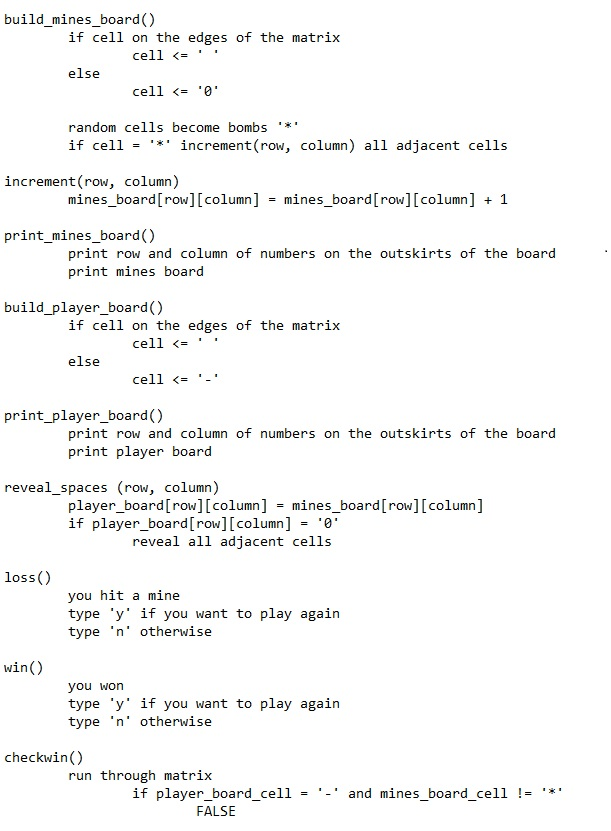
\includegraphics[scale=0.76]{1}
\label{fig:universe}
\end{figure}

\pagebreak
\begin{figure}[h!]
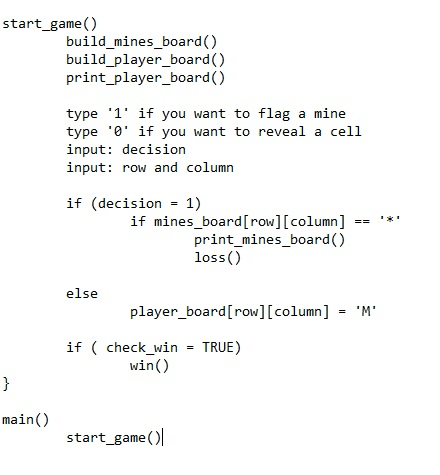
\includegraphics[scale=1]{2}
\label{fig:universe}
\end{figure}


\pagebreak
\begin{figure}[h!]
\caption{MineSweeper - auto-solver}
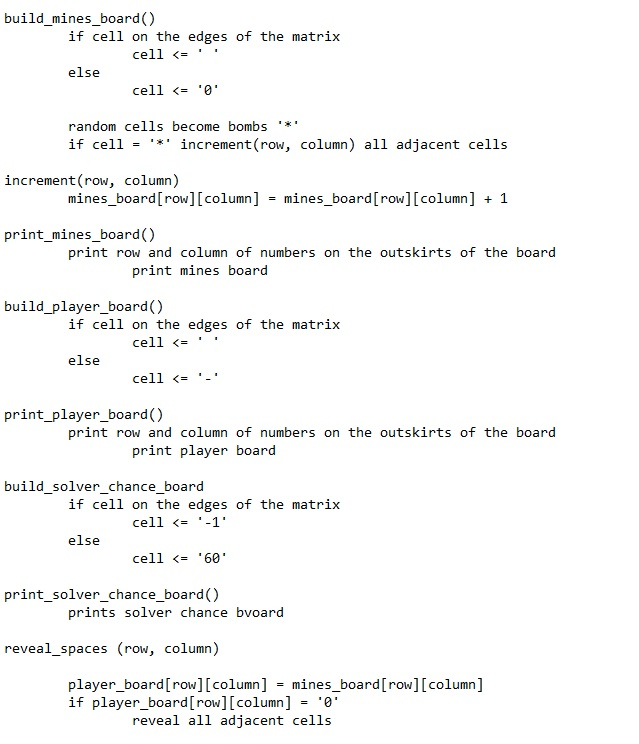
\includegraphics[scale=0.8]{3}
\label{fig:universe}
\end{figure}

\pagebreak
\begin{figure}[h!]
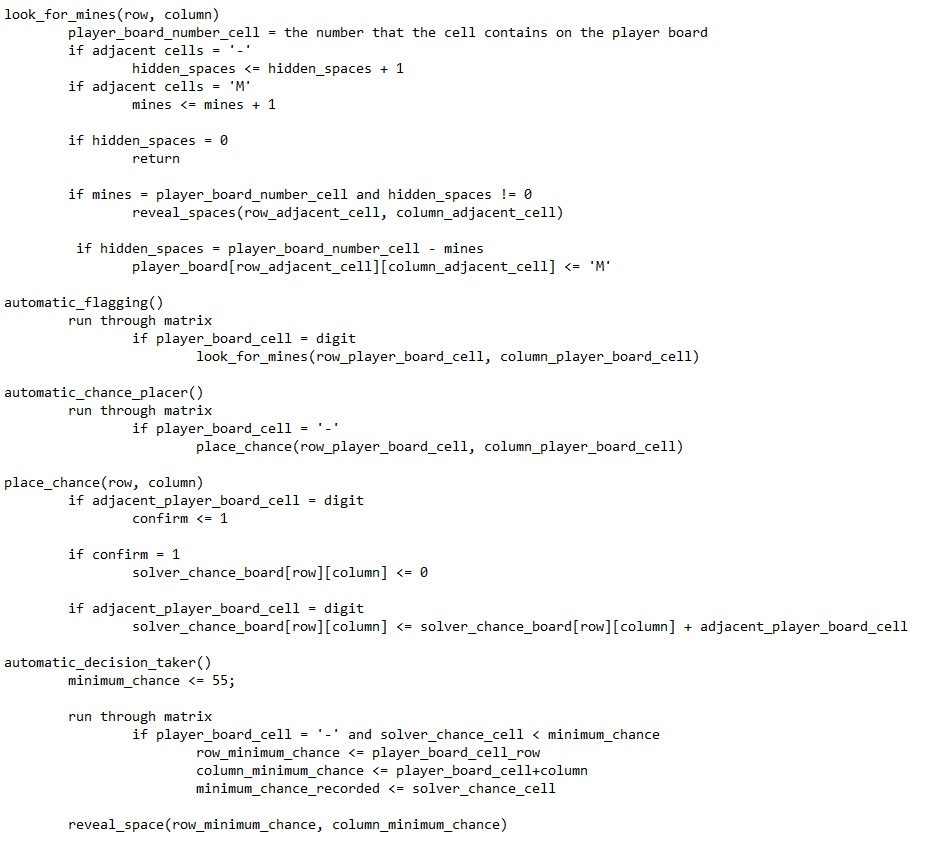
\includegraphics[scale=0.69]{4}
\label{fig:universe}
\end{figure}

\pagebreak
\begin{figure}[h!]
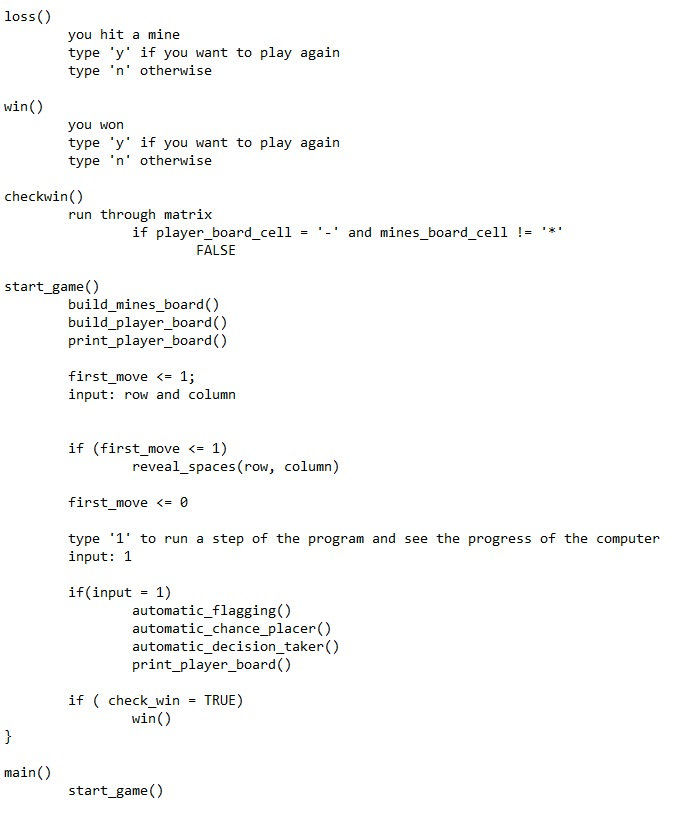
\includegraphics[scale=0.8]{5}
\label{fig:universe}
\end{figure}



\begin{thebibliography}{9}

\bibitem{latex}
\url{https://drive.google.com/file/d/0B0qJvJ1d8F8Ea0JsZ2lYUVYwR1k/view}
\bibitem{latex}
\url{https://www.youtube.com/watch?v=4aqUG5s-OEc}
\bibitem{latex}
\url{https://en.wikipedia.org/wiki/Microsoft_Minesweeper}
\bibitem{latex}
\url{https://magnushoff.com/minesweeper/}

\end{thebibliography}


\end{document}


